%%%%%
% Compile with:

%Option 1:
%1)  pdflatex Sample_Lwarp_Xy-jax.tex (possibly twice) : creates Sample_Lwarp_Xy-jax.pdf  (usual pdf file) and Sample_Lwarp_Xy-jax_html.tex. (And some other aux files.)
%2) lwarpmk html (compiles  Sample_Lwarp_Xy-jax_html.tex into Sample_Lwarp_Xy-jax_html.html and Sample_Lwarp_Xy-jaxl.html, latter possibly split.

%% The following steps are only needed once (any time tikz figures change). Only needed with tikz.
% 3) lwarpmk limages  : If there are images done with tikz, tikz-cd, etc. 
% 4) Repeat 3 and 4 (to finish creating the images)

% Sometimes  bibtex for the ``_Lwarp_Xy-jax_html.aux''  and  pdflatex Sample_Lwarp_Xy-jax_html.tex are required.


\documentclass[a4paper,12pt]{article}

%Use the next option for a stand-alone HTML file.%
%
\usepackage[mathjax]{lwarp}

%Use the next option to split html home page into subpages. Code is from https://people.bath.ac.uk/feb/lwarp/lwarp-intro.html
% %
%
% \usepackage[
%    HomeHTMLFilename= Sample_Lwarp_Xy-jax-split-index,     %  Sample_Lwarp_Xy-jax_Split =  Filename of the homepage.
%    HTMLFilename={ Sample_Lwarp_Xy-jax-},       %  Sample_Lwarp_Xy-jax- = Filename prefix of other pages.
%    mathjax                     % Use MathJax to display math.
% ]{lwarp}
% \boolfalse{FileSectionNames}     % If false, numbers the files.
% \setcounter{tocdepth}{2}         % Include subsections in the \TOC.
% \setcounter{secnumdepth}{3}      % Number down to subsections.
% \setcounter{FileDepth}{2}        % Split \HTML\ files at subsubsections
% \booltrue{CombineHigherDepths} % Combine parts/chapters/sections
% \setcounter{SideTOCDepth}{2}     % Include subsections in the side\TOC
% \HTMLTitle{Lwarp-xyJax } % Overrides \title for the web page.



\HTMLLanguage{en-UK}             % Sets the HTML meta language

%%More options
% %\HTMLTitle{ } % Overrides \title for the web page.
% %\HTMLAuthor{ }       % Sets the HTML meta author tag.
% %\HTMLDescription{ }% Sets the HTML meta description.



%%%%%%%%%%%
%% Only use if using Xy-matrix. This command line tweaks The default MATHJAX script  used by lwarp when using MATHJAX, so that browsers can find Xy-jax.
% The nature of the modifications (by Joao Faria Martins) is shown in the file.
%Modified under items 5 and 6 of licence https://www.ctan.org/license/lppl1.3
%% Original file is lwarp_mathjax.txt (automatically created bylwarp v0.902)


%\usepackage[all]{xy}
\usepackage[all,2cell,knot]{xy}
\UseAllTwocells
\MathJaxFilename{lwarp-with-Xy-jax_v3.txt}


% For original lwarp use comment out command above. Or use:

%\MathJaxFilename{lwarp_mathjax.txt}

%%%%%%%%%%%%%%%%%%%%%%%%%%%%%%%%%%%%%% If you want to modify the CSS files automatically used. use this:

%Uncomment one of the options (or leave all commented for default options).
%\CSSFilename{lwarp.css}  % automatically created by lwarpmk 
%\CSSFilename{lwarp_formal.css} % automatically created by lwarpmk  
%\CSSFilename{lwarp_sagebrush.css} % automatically created by lwarpmk 
%\CSSFilename{my_file_split.css} % Sans serif option
\CSSFilename{my_file_stand-alone.css} %margins adjusted.


%%%%%%%%%%%%%%%%%%%%%%%%%%%%%%%%%%%%%%%

\usepackage{tikz}
\usepackage{tikz-cd}

\usepackage[english]{babel} %Use this option to set the language of the document.
\usepackage[utf8]{inputenc}

\usepackage{hyperref}

\usepackage{amssymb}

\usepackage{amscd}

\usepackage{caption}

\usepackage[normalem]{ulem}



\usepackage{geometry}
\geometry{verbose,tmargin=2.5cm,bmargin=1.5cm,lmargin=2cm,rmargin=2cm,headheight=1cm,headsep=1cm,footskip=1cm}

\usepackage{amsmath}
\usepackage{amsthm}
\newtheorem*{Note}{Note}

\newtheorem{Theorem}{Theorem}
\newtheorem{Exercise}[Theorem]{Exercise}

\newtheorem{Corollary}[Theorem]{Corollary}
\newtheorem{Lemma}[Theorem]{Lemma}
\newtheorem{Definition}[Theorem]{Definition}
\newtheorem{Notation}[Theorem]{Notation}
\newtheorem{Convention}[Theorem]{Convention}

\newtheorem{Example}[Theorem]{Example}
\newtheorem{Remark}[Theorem]{Remark}
\newtheorem{Warning}[Theorem]{Warning}
\newtheorem{Proposition}[Theorem]{Proposition}
\newtheorem{Fundamental Theorem}{Fundamental Theorem}

\newcommand{\C}{ \mathbb{C} }
\newcommand{\Cc}{ \mathcal{C} }
\newcommand{\Dc}{ \mathcal{D} }
\newcommand{\Grp}{ \mathrm{Grp} }

\newcommand{\Z}{ \mathbb{Z} }
\newcommand{\ra}[1]{\xrightarrow{#1}}
\DeclareMathOperator{\Sym}{Sym}
\def \id {\mathrm{id}}
\newcommand{\Q}{\mathbb{Q}}
\renewcommand{\a}{{\alpha}}
\renewcommand{\b}{{\beta}}
\def \g {\gamma}
\def \w {\omega}
\def \e {\epsilon}
\def \z {\zeta}
\def \d {\partial}

\newcommand{\tHpb}[3]{{\mathbf{\overline{2H}}^{#1}_{(#2,#3)}}}
\newcommand{\Hpb}{\mathbf{\overline{H}}}

\def \red{\textcolor{red}}

\def \green{\textcolor{green}}
\def \blue{\textcolor{blue}}
%% The following is how your commands and definitions will appear in the web page.
\begin{warpHTML}
\CustomizeMathJax{\newcommand{\C}{ \mathbb{C} }}
\CustomizeMathJax{\newcommand{\Cc}{ \mathcal{C} }}
\CustomizeMathJax{\newcommand{\Dc}{ \mathcal{D} }}
\CustomizeMathJax{ \newcommand{\Grp}{ \mathrm{Grp} } }
\CustomizeMathJax{\newcommand{\Z}{ \mathbb{Z} }}
\CustomizeMathJax{\newcommand{\ra}[1]{\xrightarrow{#1}}}
\CustomizeMathJax{\DeclareMathOperator{\Sym}{Sym}}
\CustomizeMathJax{\def \id {\mathrm{id}}}
\CustomizeMathJax{\newcommand{\Q}{\mathbb{Q}}}
\CustomizeMathJax{\renewcommand{\a}{{\alpha}}}
\CustomizeMathJax{\renewcommand{\b}{{\beta}}}
\CustomizeMathJax{\def \g {\gamma}}
\CustomizeMathJax{\def \w {\omega}}
\CustomizeMathJax{\def \e {\epsilon}}
\CustomizeMathJax{\def \z {\zeta}}
\CustomizeMathJax{\def \d {\partial}}

\CustomizeMathJax{\newcommand{\tHpb}[3]{{\mathbf{\overline{2H}}^{#1}_{(#2,#3)}}}}
\CustomizeMathJax{\newcommand{\Hpb}{\mathbf{\overline{H}}}}


\CustomizeMathJax{\def \red{\textcolor{red}}}

\CustomizeMathJax{\def \green{\textcolor{green}}}
\CustomizeMathJax{\def \blue{\textcolor{blue}}}
\end{warpHTML}

\begin{document}

\title{Sample HTML file: produced with  lwarp, with mathematical formulae displayed with  MathJax, and  xymatrix commutative  diagrams displayed  with XyJax-v3}
\author{Jo\~{a}o Faria Martins}
\affiliation{University of Leeds}
\date{Last modified: April 15, 2024}
\maketitle

\tableofcontents
$$\xymatrix@R=30pt@C=60pt
{&A\ar[d]_{\iota_0^A}  \ar[r]^f & X\ar[d]_{\iota_0^X} \ar[r]^g & B.\\
            & A \times I  \ar@/_4pc/[rru]_<<<<<<<<<<<{H} \ar[r]^{f \times \id_I} & X\times I \ar@{-->}[ur]^{H'} } $$
  $$\hskip-0.5cm\xymatrix@C=25pt@R=30pt{& T\times T\ar[drr]_{\sqcup} \ar[rr]^{  \tau} &\drtwocell\omit{\,\,\, \mathbf{R}}& T \times T \ar[d]^{\sqcup} \\
 &&& T.}
 $$


\noindent The responsibility for this HTML file is \href{https://joaofariamartins.github.io/}{Jo\~{a}o Faria Martins}' only.\\
Corrections, suggestions, etc. are very welcome, and can be sent to:
\href{mailto:j.fariamartins@leeds.ac.uk}{j.fariamartins@leeds.ac.uk}.\\
\textbf{This is strictly a non-specialist experimental file.} \\


See the links below for:
\begin{itemize}
   \item \href{Sample_Lwarp_Xy-jax.html}{``stand-alone'' version of this webpage},
   \item \href{Sample_Lwarp_Xy-jax-split-index.html}{``split'' version of this webpage} (with sans serif fonts),
    \item \href{Sample_Lwarp_Xy-jax.pdf}{pdf version of this page},
   \item Latex source for the stand alone version of this page \href{Sample_Lwarp_Xy-jax.tex}{Sample\_Lwarp\_Xy-jax.tex},
    \item Latex source for the split version of this page, with sans serif fonts: \href{Sample_Lwarp_Xy-jax-split.tex}{Sample\_Lwarp\_Xy-jax-split.tex},
   \item CSS files for the stand-alone version of this page: \href{lwarp.css}{lwarp.css} (automatically provided by \emph{lwarpmk}) and \href{my_file_stand-alone.css}{my\_file\_stand-alone.css} (minor tweak to adjust margins),
   \item CSS files for the split version of this page: \href{lwarp\_formal.css}{lwarp\_formal.css} (automatically provided by \emph{lwarpmk}) and \href{my_file_split.css}{my\_file\_split.css} (minor tweak enforcing sans serif fonts).
   \item Configuration file required for browsers to find Xy-Jaxv3,
\href{lwarp-with-Xy-jax_v3.txt}{lwarp-with-Xy-jax\_v3.txt}. This script is essentially the original Lwarp MathJax emulation code, \href{lwarp_mathjax.txt}{lwarp\_mathjax.txt}  (automatically created by  lwarp v0.902), with two minimal additions, as shown.
\end{itemize}


\section{Context and instructions: using Lwarp to compile latex to HTML, so that xymatrix diagrams are displayed with Xy-Jax}\label{Context}

\noindent This HTML file (that you are reading) was produced with the
\href{https://ctan.org/pkg/lwarp}{lwarp.sty package}, available with \textbf{TeXLive}.
\medskip
\footnote{See also \url{https://people.bath.ac.uk/feb/lwarp/lwarp-intro.html}, for a quick introduction on how to use Lwarp, and without which this explanation that you are reading would not have been written.}
\medskip
In particular the preamble contains:
\begin{verbatim}
\documentclass[a4paper,12pt]{article}
\usepackage[mathjax]{lwarp}
\end{verbatim}

\medskip
The version of the software was:
\begin{verbatim}
 pdfTeX, Version 3.141592653-2.6-1.40.24 (TeX Live 2022) (preloaded format=pdflatex)
 lwarpmk: lwarpmk: v0.910  Automated make for the LaTeX Lwarp package.
\end{verbatim}

The source latex file can be found here: \href{Sample_Lwarp_Xy-jax.tex}{Sample\_Lwarp\_Xy-jax.tex}  or here \href{Sample_Lwarp_Xy-jax-split.tex}{Sample\_Lwarp\_Xy-jax-split.tex}, depending whether you are seeing the  \href{Sample_Lwarp_Xy-jax.html}{``stand-alone'' version of this webpage}, or the
   \href{Sample_Lwarp_Xy-jax-split-index.html}{``split'' version of this webpage}.


\

 \noindent This HTML file  also makes use of the following configuration script, so that {\textbf{Xy-pic}} diagrams, particularly \href{https://www.ctan.org/pkg/xymatrix}{\textit{xymatrix}} commmutative diagrams, can be displayed by using \textbf{Xy-Jax-v3}. (Or at least a good sample  of them: there seem to be some compatibility issues.)\\
\begin{center}
\href{lwarp-with-Xy-jax_v3.txt}{lwarp-with-Xy-jax\_v3.txt}.
\end{center}
This script file has minimal additions (two in total) in the original Lwarp MathJax emulation code, that is automatically created by  lwarp v0.902), namely:
\begin{center} \href{lwarp_mathjax.txt}{lwarp\_mathjax.txt}, \end{center}
 (Two lines were added to the script above, as shown,  in order that browsers can find Xy-Jaxv3.)

\noindent This modification was produced under items 5 and 6 of the licence \url{https://www.ctan.org/license/lppl1.3}  (The LATEX Project Public License 1.3).
\\
Credit is  due to instructions in: \url{https://github.com/sonoisa/XyJax-v3} (the official Xy-Jaxv3 documentation) and in  "40.11 lwarp\_mathjax.txt" of the \href{http://mirrors.ibiblio.org/CTAN/macros/latex/contrib/lwarp/lwarp.pdf}{official Lwarp documentation}.


\bigskip

 If using \Xy-pic diagrams displayed with {\textbf{XyJax-v3}}, insert the following in the preamble of your latex file:
\begin{verbatim}
  \usepackage[all]{xy}
  \MathJaxFilename{lwarp-with-Xy-jax_v3.txt}
\end{verbatim}


\textbf{Compile .tex to .html using:}

\begin{enumerate}
 \item  \emph{pdflatex Sample\_Lwarp\_Xy-jax.tex} (possibly twice) : creates Sample\_Lwarp\_Xy-jax.pdf  (usual pdf file, that can also be shared) and Sample\_Lwarp\_Xy-jax\_html.tex. (And some other aux files.)
\item  \emph{lwarpmk html} : converts Sample\_Lwarp\_Xy-jax\_html.tex  to Sample\_Lwarp\_Xy-jax\_html.html. And then creates Sample\_Lwarp\_Xy-jax.html (possibly split into different HTML files if such option is chosen).
\item[] \qquad \textbf{Note:} Use \emph{lwarpmk html1} to force a recompile.
\item[] \qquad \textbf{Note:} In case of error, with \emph{lwarpmk html}, use \emph{lwarpmk pdftohtml} to create HTML file.
\item[] \qquad \textbf{Note:} When using \emph{bibtex} files, then the following is required:  \begin{itemize}\item  bibtex  {Sample\_Lwarp\_Xy-jax\_html.aux} \item \emph{pdflatex} Sample\_Lwarp\_Xy-jax\_html.tex\end{itemize}

\item[] The following steps are only needed once (any time tikz figures change). Only needed with tikz.
\item  \emph{lwarpmk limages}  : If there are images done with tikz, tikz-cd, etc.
\item  Repeat 2 (now using \emph{lwarpmk html1}) and 3 (to finish creating the images).
\end{enumerate}
\begin{Note}It is advisable to use a recent version of \emph{\textbf{TexLive}.}\end{Note}




\textbf{Warnings:}
\begin{itemize}
  \item  The usage of  \href{https://github.com/sonoisa/XyJax-v3}{\textbf{XyJax-v3}} software with \href{https://ctan.org/pkg/lwarp}{lwarp} is experimental.
  \item Not all accessibility features of commutative diagrams displayed with XyJax-v3 work.\\ Among the accessibility features that seem to work well are:
 \begin{enumerate}
  \item View original latex source.
  \item Zoom maths expression.
 \end{enumerate}
 \end{itemize}






\section{Examples: xymatrix diagrams displayed with Xy-Jaxv3 using Lwarp}\label{sec:context}

This is an example of a HTML file with:
\begin{itemize}
\item Mathematical formulae displayed with  \href{https://www.mathjax.org/}{\textbf{MathJax}}:
\begin{equation}\label{test}
   x^2+y^2=1,
\end{equation}
$$\big ( x \ra{ \gamma } y\big) \in \pi_1(X,X_0),
$$
$$
\dots \to \pi_i(E_b,x) \ra{\iota} \pi_i(E,x) \ra{\d}  \pi_i(B,b) \ra{\delta}  \pi_{i-1}(E_b,x) \to \dots
 \ra{\iota} \pi_1(E,x) \ra{\partial}  \pi_1(B,b) \ra{\delta_x} \pi_0(E_b) \ra{\iota} \pi_0(E)=\{0\}.
$$
% \begin{multline*}\Gamma(h,Q)=\Gamma \big (\Q(\w,\a,\z,\e):\Q )  \ge  \Gamma \big (\Q(\w,\a,\z,\e): \Q(\omega)\big)   \ge  \Gamma\big (\Q(\w,\a,\z,\e), \Q(\w,\a) \big ) \\ \ge \Gamma \big (\Q(\w,\a,\z,\e), \Q(\w,\a,\z) \big ) \ge  \Gamma\big (\Q(\w,\a,\z,\e),\Q(\w,\a,\z,\e)\big )=\{e\}. \end{multline*}

\item To see how lecture notes look like with Lwarp, see subsections \ref{adjunctions} and \ref{Galois}.
\item 
This configuration is compatible with AMS-CD commutative diagrams, e.g. this diagram from the \href{https://www.jmilne.org/not/Mamscd.pdf}{amscd package manual}:
\[
\begin{CD}
A @>a>b> B\\
@VlVrV @AlArA\\
C @<a<b< D
\end{CD}
\]\begin{quotation}
  \end{quotation}

\item  Commutative diagrams drawn with \href{https://tug.org/applications/Xy-pic/}{\textbf{Xy-pic}} displayed by using \href{https://github.com/sonoisa/XyJax-v3}{\textbf{XyJax-v3}}.\\
For a good introduction to typeseting diagrams with Xy-pic see e.g.
\begin{itemize}
 \item \url{https://www.math.purdue.edu/~adebray/lecture_notes/using_xy.pdf} (Arun Debray
Using \Xy\ to typeset automata.
July 5, 2016.)


\item \url{https://web.math.ku.dk/~holm/download/xyrefer.pdf} (Kristoffer H. Rose \&
Ross Moore: \Xy-pic Reference Manual, Version 3.7 1999/02/16.)

\item See also the more recent \href{https://anorien.csc.warwick.ac.uk/mirrors/CTAN/macros/generic/diagrams/xypic/doc/xyguide.pdf}{user guide} (Kristoffer H. Rose,
Version 3.8.9, October 6, 2013) in the official page of \href{https://ctan.org/pkg/xymatrix?lang=en}{xymatrix – Commutative diagrams using XY-pic
}
\end{itemize}


E.g.$$\xymatrix@R=60pt@C=60pt{&S_3 \ar@{^{(}->}[r]^f \ar[dr]_{g}^{\cong} &S_4 \ar@{->>}[d]^\pi \\
&&S_4/V,
}
$$

\[
\xymatrix{ && \Q\\ 
& \Q(\w) \ar@{<-}[ur] \\ & & \Q(\g)\ar@{<-}[uu] & \Q(\b)\ar@{<-}[uul] & \Q(\a),\ar@{<-}[uull]\\
&&\Q(\a,\b,\g)\ar@{<-}[uul]\ar@{<-}[u] \ar@{<-}[ur] \ar@{<-}[urr]
} 
\] 

$$\xymatrix@R=1pt{\\\\\\(123).}\xymatrix@R=39pt{ & \red{\bullet}\ar@{-}[dr]  \ar@{-}[rr] && \blue{\star}\ar@{-}[dl] \\
                && \green{\square} }\qquad\xymatrix@R=1pt{\\\\\\\\ =}
\xymatrix@R=39pt{ & \blue{\star}\ar@{-}[dr]  \ar@{-}[rr] && \green{\square}\ar@{-}[dl] \\
                && \red{\bullet} }  \xymatrix@R=1pt{\\\\\\\\ ,}$$

$$\xymatrix@R=30pt@C=60pt
{&A\ar[d]_{{\iota_0}^A}  \ar[r]^f & X\ar[d]_{{\iota_0}^X} \ar[r]^g & B,\\
            & A \times I  \ar@/_4pc/[rru]_<<<<<<<<<<<{H} \ar[r]^{f \times \id_I} & X\times I \ar@{-->}[ur]^{H'} } $$


 $$
\xymatrix
{ &  \displaystyle \bigoplus_{y \in H_0}  \mathbf{H}_1(x,y)\otimes\mathbf{H}_1'(y,z)\ar[dd]_{\displaystyle \bigoplus_{y \in H_0} \eta_{(x,y)} \otimes \eta'_{(y,z)}}  \ar[rr]^{\mathrm{proj}} && \displaystyle  \int^{y \in H_0} \mathbf{H}_1(x,y)\otimes\mathbf{H}_1'(y,z)\ar@{-->}[dd]^{ \displaystyle \int^{y \in Y}   \eta_{(x,y)} \otimes \eta'_{(y,z)} }\\
\\
& \displaystyle \bigoplus_{y \in H_0}  \mathbf{H}_2(x,y)\otimes\mathbf{H}_2'(y,z)  \ar[rr]_{\mathrm{proj}} && \displaystyle \int^{y \in H_0} \mathbf{H}_2(x,y)\otimes\mathbf{H}_2'(y,z)\,\, ,
}
$$
$$\xymatrix{
&\displaystyle\int^{y \in {Y}} \Hpb_{(X,Y)}^{M_1}(-,y) \otimes \Hpb_{(Y,Z)}^{M_2}(y,-)\ar@{=>}[dd]|{\tHpb{\mathbf{W}_1}{X}{Y} \bullet \tHpb{\mathbf{W}_2}{Y}{Z}}
\ar@{=>}[rrr]^>>>>>>>>>>>>>>>>>{\eta_{(X,Y,Z)}^{M_1,M_2}}&&& \Hpb_{(X,Z)}^{M_1\times_Y M_2}
\ar@{=>}[dd]|{\tHpb{\mathbf{W}_1\#_0 \mathbf{W}_2}{X}{Z}}
\\\\
&\displaystyle\int^{y \in {Y}} \Hpb_{(X,Y)}^{N_1}(-, y) \otimes \Hpb_{(Y,Z)}^{N_2}(y,-)\ar@{=>}[rrr]^>>>>>>>>>>>>>>>>>{\eta_{(X,Y,Z)}^{N_1,N_2}}&&& \Hpb_{(X,Z)}^{N_1\times_Y N_2}\,. }
$$



        $$\xymatrix{ &\Cc\rtwocell^F_{F'}{\eta} &\Dc } $$


$$\hskip-0.5cm\xymatrix@C=25pt@R=30pt{& T\times T\ar[drr]_{\sqcup} \ar[rr]^{  \tau} &\drtwocell\omit{\,\,\, \mathbf{R}}& T \times T \ar[d]^{\sqcup} \\
 &&& T.}
 $$

  $$\xymatrix@C=45pt{&\Cc \sqcup \Cc' \rtwocell\omit{\quad \,\, \langle\eta,\eta'\rangle}
  \ar@/^1.5pc/[r]^{T_b\circ \langle f, f' \rangle}
    \ar@/_1.5pc/[r]_{\langle T,T'\rangle} & \Grp.  }$$

$$
\xymatrix@C=60pt{\Cc\ruppertwocell^F{\eta}
\rlowertwocell_{F''}{\eta'}
\ar[r]|{F''} & \Dc  & = &\Cc\ar@/^1.5pc/[r]^{F}\ar@/_1.5pc/[r]_{F''}\rtwocell\omit{\quad\,\,\,\,\eta\#_1\eta'}
  & \Dc &}
$$
 $$
\hskip-2cm\xymatrix@C=60pt{ &\big( \mathbf{Cob}^{(n,n+1,n+2)}\big)^3
\ar[d]_{\id\times \sqcup}\ar[dr]^{\sqcup\times \id}
 \drrtwocell
 \omit
 {\qquad \boldsymbol{\chi}'\times \mathcal{F}_{\mathbf{B}}}
 \ddtwocell\omit{<-13> \alpha}
\ar[rr]^{\mathcal{F}_{\mathbf{B}} \times \mathcal{F}_{\mathbf{B}} \times \mathcal{F}_{\mathbf{B}}}
&& \big(\mathbf{Prof} \big)^3\ar[d]^{\otimes \times \id}\\
&\big( \mathbf{Cob}^{(n,n+1,n+2)})^2 \ar[d]_{\sqcup}
& \big( \mathbf{Cob}^{(n,n+1,n+2)})^2 \ar[dl]^{\sqcup}
 \dtwocell
 \omit
 { \boldsymbol{\chi}'}
\ar[r]^{\mathcal{F}_{\mathbf{B}} \times \mathcal{F}_{\mathbf{B}}}
&  \big(\mathbf{Prof} \big)^2
\ar[dl]^{\otimes}
\\
& \big(\mathbf{Cob}^{(n,n+1,n+2)}\big) \ar[r]_{\mathcal{F}_{\mathbf{B}}}& \mathbf{Prof}\\
& \ar@3[r]_{\boldsymbol{\omega}'} & \\ &\big( \mathbf{Cob}^{(n,n+1,n+2)}\big)^3
\ar[d]_{\id\times \sqcup} \drrtwocell\omit{\quad \qquad \mathcal{F}_{\mathbf{B}}\times \boldsymbol{\chi}' }\ar[rr]^{\mathcal{F}_{\mathbf{B}} \times \mathcal{F}_{\mathbf{B}} \times \mathcal{F}_{\mathbf{B}}} && \big(\mathbf{Prof} \big)^3\ddltwocell\omit{\alpha}
\ar[d]^{\otimes \times \id}\ar[dl]^{\id\times \otimes}\\
&\big( \mathbf{Cob}^{(n,n+1,n+2)})^2 \ar[d]_{\sqcup} \drtwocell\omit{\,\,\boldsymbol{\chi}' } \ar[r]^{\mathcal{F}_{\mathbf{B}} \times \mathcal{F}_{\mathbf{B}}}   & \big( \mathbf{Prof})^2
   \ar[d]^{\otimes}
 &  \big(\mathbf{Prof} \big)^2\ar[dl]^{\otimes}\\
& \big(\mathbf{Cob}^{(n,n+1,n+2)}\big) \ar[r]_{\mathcal{F}_{\mathbf{B}}}& \mathbf{Prof}.
}
$$


\end{itemize}


\section{Issues when using XyJax-v3 and Lwarp for typesetting xymatrix diagrams}
Please do contact me if you know the solution to any of these issues. Remember: this is stricly a non-specialist file!



\begin{itemize}
\item The commands of the form:
\begin{verbatim} \stackrel{(*)}{\implies} \end{verbatim}
or
\begin{verbatim}\left ( x \xrightarrow{f} y\right) \end{verbatim}
do not seem to work well inside
\begin{verbatim} \begin{equation} \end{equation}. \end{verbatim}
So use instead, for example,
\begin{verbatim}$$ \stackrel{(*)}{\implies} $$ \end{verbatim}
\begin{verbatim}$$ \left ( x \xrightarrow{f} y \right)$$\end{verbatim}.
Here is how it looks:
$$ \stackrel{(*)}{\implies}$$
$$\left ( x \xrightarrow{f} y \right) .$$

\item Sometimes there are errors if there are mathematical commands in the title of sections, subsections, etc.
\item Lwarpmk gives error messages if it finds \textit{xymatrix} inside:
\begin{verbatim} \begin{equation} \end{equation}. \end{verbatim}
(However a html file can still be produced with \textit{lwarpmk pdftohtml}.)

\medskip

\noindent So avoid: \begin{verbatim} \begin{equation} \xymatrix{    } \end{equation}, \end{verbatim}
and use instead:
 \begin{verbatim} \[ \xymatrix{   } \], \end{verbatim}
 or
  \begin{verbatim} $$ \xymatrix{   } $$. \end{verbatim}


  \item  \textbf{Not all accessibility functions of MathJax work with Xy-Jaxv3, only some can be used, e.g. zoom and source latex code}.\\
Accessibility features of  Xy-jax \href{https://github.com/sonoisa/XyJax-v3}{are not  officially supported}.\\

\item References to section, chapters etc, have glitches \textbf{if inside mathematics environments}. For instance, the links provided do not appear to work well. E.g.
\begin{equation}\label{Euler}
 \exp(x+yi)=e^x\big (\cos(y)+i\sin(y) \big)
\end{equation}
\begin{align*}
 e^{i\pi}+1&=\big(\cos(\pi)+i\sin(\pi) \big)+1, \quad \textrm{ using Equation }  \eqref{Euler}.  \textrm{ (Just for testing) equations } \eqref{test}, \eqref{xydiagram}\\
           &=0. \quad \textrm{ A reference to second section } \protect \ref{sec:context}
\end{align*}
Outside maths environments all seems to work fine:
  \begin{quotation} Using  Equation   \eqref{Euler}.   (Just for testing) equations  \eqref{test}, \protect{\eqref{xydiagram}}\\  A reference to second section  \protect{\ref{sec:context}}
  \end{quotation}
\item When compiling xymatrix, or tikz, diagrams as sgv figures, with Alt-Text (which sometimes is necessary) it sometimes happens that the figure is not cropped correctly. This seems to depend stronly on the operating system being used.
\end{itemize}
\section{More general notes}
\begin{itemize}


\item \textbf{pdf} and \textbf{HTML} automatically coexist: here is the pdf version  of this HTML file \href{Sample_Lwarp_Xy-jax.pdf}{Sample\_Lwarp\_Xy-jax.pdf}

\item It is possible to split an HTML page into sub-pages: credit \url{https://people.bath.ac.uk/feb/lwarp/lwarp-intro.html}. Instructions can be seen in the source latex file of this HTML file  \href{Sample_Lwarp_Xy-jax.tex}{Sample\_Lwarp\_Xy-jax.tex}.

 \item Additions are required in the .tex file in order that \textbf{MathJax} displays commands, macros and definitions correctly.
        E.g. write:
\begin{verbatim}
\DeclareMathOperator{\Sym}{Sym}
\def \Mon {{\mathbf{Mon}}}
\newcommand{\Q}{\mathbb{Q}}
\end{verbatim}

and then:

\begin{verbatim}
\begin{warpHTML}
  \CustomizeMathJax{\DeclareMathOperator{\Sym}{Sym}}
  \CustomizeMathJax{\def \Mon {{\mathbf{Mon}}}}
  \CustomizeMathJax{\newcommand{\Q}{\mathbb{Q}}}
\end{warpHTML}
\end{verbatim}
This means that you can use slightly different versions of commands for pdf and for html.
\item If using Xy-pic diagrams (if displayed as Xy-jax) put in the preamble of the tex file:
\begin{verbatim}
 \MathJaxFilename{lwarp-with-Xy-jax_v3.txt}
\end{verbatim}
You will also need this configuration file: \href{lwarp-with-Xy-jax_v3.txt}{lwarp-with-Xy-jax\_v3.txt}.
(Explanation is in Section \ref{Context}.)


\item Sample use of Xy-pic compatible with lwarp (so that the resulting xymatrix code  is readable by Xy-Jax):
E.g.:
\begin{verbatim}
\[
\xymatrix
{
&& \Q\\ & \Q(\w) \ar@{<-}[ur] \\
& & \Q(\g)\ar@{<-}[uu] & \Q(\b)\ar@{<-}[uul] & \Q(\a)\ar@{<-}[uull]\\
&&\Q(\a,\b,\g)\ar@{<-}[uul]\ar@{<-}[u] \ar@{<-}[ur] \ar@{<-}[urr]
}
\],
\end{verbatim}
or
\begin{verbatim}
\displaymathnormal{$$
\xymatrix{
&S_3 \ar@{^{(}->}[r]^f \ar[dr]_{g}^{\cong} &S_4 \ar@{->>}[d]^\pi
\\ &&S_4/V,
}
$$}.
\end{verbatim}


 \item Figures, with alternative text, can be included like this:

\begin{verbatim}
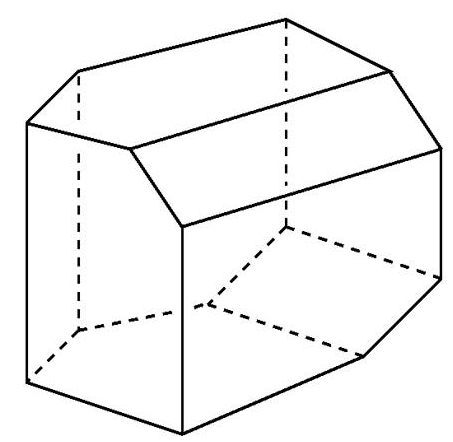
\includegraphics[width = 0.4\textwidth,
alt={Type your alternative text here}]{Stasheff.png}
\end{verbatim}

\begin{center}{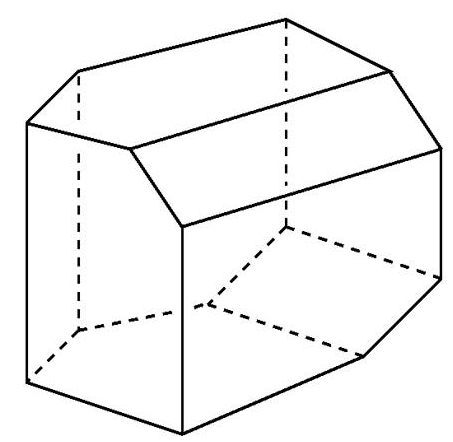
\includegraphics[width = 0.3\textwidth,alt={This figure shows Stasheff's Polytope. The top face is a pentagon, the bottom face is a pentagon ... }]{Stasheff.png}}
\end{center}






\item Figures, including \textbf{tikz} and \textbf{tikz-cd figures}, can be compiled as figures with \textbf{Alt Text}. (The same option is  also available for xymatrix diagrams, and may be preferable to Xy-Jaxv3, in the cases when it is sensible to provide a comprehensive alternative text to the figure/diagram, instead of relying mainly on the availability of the latex code, for accessibility.)\\
\textbf{Warning:} In some operating systems, issues seem to exist with the conversion of tikz figures to svg: e.g. figures may be incorrectly cropped for the web-page. \\ Size of xymatrix figures and tikz-cd figures seemingly then must be adjusted manually.



\item        When using \textbf{tikz} pictures use (note the Alt Text option):
\begin{verbatim}
\begin{figure}\ThisAltText{Alt text to your diagram}
\begin{tikzpicture} 

\end{tikzpicture}
\end{figure}
\end{verbatim}
or
\begin{verbatim}
\begin{center}\ThisAltText{Alt text to your diagram}
\begin{tikzpicture}

\end{tikzpicture}
\end{center}
\end{verbatim}

Examples  can be found towards the end of this file.
\item When using \textbf{tikz-cd} use:
\begin{verbatim}
{\displaymathother
 \ThisAltText{ Alt text to your commutative diagram }
\[
     \begin{tikzcd} F(A) \arrow{r}{F(f)}& F(B) \\
     G(A)\arrow{r}[swap]{G(f)} \arrow{u}{\eta_A} & G(B)
     \arrow{u}[right]{\eta_B}
     \end{tikzcd}
\]
} 
\end{verbatim}
 


\item It is possible to compile an \textbf{Xy-pic diagram} as a \textbf{figure with alt text}. Use:
\begin{verbatim}
{
\displaymathother
\ThisAltText{Write some alt text here.}
$$ \xymatrix{ } $$
}
\end{verbatim}
  Examples  can be found towards the end of this file.


\item \textbf{To select your own  .CSS files use:}
\begin{verbatim}
 \CSSFilename{your_file.css}
\end{verbatim}

\item  Avoid good old Tex commands like 
\begin{verbatim} {\bf }, {\it }.\end{verbatim}

It seems that lwarp does not deal with them properly. Instead use: 
\begin{verbatim} \textbf{ }, \textit{ }.\end{verbatim}
(In fact better to avoid \textit{italics} altogether for accessibility reasons: use \textbf{bold}.) 
\item Lwarp  gives  errors messages when compiling  Xy-pic diagrams  inside
\begin{verbatim} \begin{equation} \end{equation}\end{verbatim}
Use instead:
\begin{verbatim}
\[\xymatrix{} \]
or
\[\begin{xy} \xymatrix{} \end{xy}\]
\end{verbatim}
Or use \emph{lwarpmk pdftohtml} if there are compilation errors.

\item Figures created with tikz and xymatrix frequently have issues: e.g. they may be too small (so size needs to be adjusted), or incorrectly cropped. Seems to depend on operating system.
\end{itemize}



\bigskip
\section{Some examples of tikz and xymatrix diagrams compiled as svg images, with alternative text}

As written in Section \ref{sec:context}, it is possible to display xymatrix diagrams by using XyJax-v3. In some cases, it may however be preferable to compile xymatrix diagrams as figures with \textbf{Alt Text}. (E.g. it may be sensible to instead provide a comprehensive alternative text to the figure/diagram, instead of relying mainly on the availability of the latex code, for accessibility.)\\

This option (svg image with alternative text) is also available for tikz and tikz-cd figures. Examples are below.

\subsection{An xymatrix diagram compiled as an image with alt text}\label{xymatrix-with-alttext}
An \textit{xymatrix} diagram compiled into a picture with alt text. Can utilize equation numbers, with no errors. The size of the svg image must be adjusted. Sometimes the image is not correctly cropped: depends on operating system.
{\displaymathother
 \ThisAltText{This diagram shows a right triangular, diagram, with the top side horizontal, being a cathet, and containing an arrow $\tau$, from $T\times T$ to $T\times T$. From the right-hand-end of the cathet,  there is vertical downwards arrow (also a cathet), $\sqcup\colon T\times T \to T$. From the left-hand-side of the initial cathet, there is the hypothese downwards arrow marked with $\sqcup\colon T\times T \to T$. There is a 2-cell from the composition of the two cathets to the hypothese, marked with boldface $R$}
\begin{equation}\label{xydiagram}
\xymatrixcolsep{0.5cm}\xymatrixrowsep{2cm}\hskip-0.5cm\xymatrix{& T\times T\ar[drr]_{\sqcup} \ar[rr]^{  \tau} &\drtwocell<\omit>{\,\,\, \,\,\,\mathbf{R}}& T \times T \ar[d]^{\sqcup} \\
 &&& T.}
\end{equation}
}



\subsection{A tikz image compiled as an image with alt text:}
Size can be adjusted.  Sometimes (depending on operating system, it seems) the image may be incorrectly cropped. See figure \ref{fig:triangle}.
\begin{center}
\begin{figure}[ht!]
\ThisAltText{An equilateral triangle, with one of the edges horizontal. Vertices are labelled 1, 2 and 3, clockwise, starting from the top left vertex.}
\centering
\begin{tikzpicture}[scale=1]
\draw[-][very thick] (5,0)  -- (10,0);
\draw[-][very thick] (5,0)  -- (7.5,-4);
\draw[-][very thick]  (7.5,-4) -- (10,0);
\node at (4.7,0) {$1$};
\node at (10.3,0) {$2$}; 
\node at (7.5,-4.3) {$3$};
\end{tikzpicture}
\caption{An equilateral triangle with its vertices labeled 1, 2 and 3}
\label{fig:triangle}
\end{figure}
 \end{center}
 \subsection{A tikz image compiled to an image with alt text, outside a float environment}

\begin{center}
 \ThisAltText{This figure shows a rectangle, whose largest side is horizontal.
 Is vertices are labelled  1, 2 (top edge) and  3 and 4. (bottom edge), from left to right.}
\begin{tikzpicture}[scale=0.7]
\draw[-][very thick] (5,0)  -- (15,0);
\draw[-][very thick] (5,0)  -- (5,-4);
\draw[-][very thick]  (5,-4) -- (15,-4);
\draw[-][very thick]  (15,-4) -- (15,0);
\node at (4.5,0) {$1$};
\node at (15.5,0) {$2$};
\node at (4.5,-4.5) {$3$};
\node at (15.5,-4.5) {$4$};
\end{tikzpicture}
 \end{center}

\subsection{A tikz image compiled to an image with alt text, outside a float environment, and with a caption}

 \begin{center}\ThisAltText{The figure shows two disks, $A$ and $B$, of the same radius, centered at points, on a horizontal line. The radii are smaller than the distance between the center points, but greater than half of the distance. The intersection of the two disks is called $C$. There is a point $x \in A\cap B$, and another disk, $D$, centered in $x$ and contaned in $A\cap B$. }
\begin{tikzpicture}[scale=0.5,very thick]
\node at (0,0) [shape=circle,draw,inner sep=40pt, fill=green!50!white, opacity=0.2, dashed]{};
\node at (5,0) [shape=circle,draw,inner sep=30pt, fill=red!50!white, opacity=0.2, dashed]{};
\node at (3,0.4) [shape=circle,draw,inner sep=08.5pt, fill=gray!50!white, opacity=0.5, dashed]{};
\node at (3,0.4) {$\bullet$};
\node at (3,0.9) {$x$};
\node at (3,-1.1) {$C$};
\node at (-0.5, -3) {\small $A$};
\node at (5.6, -2) {\small $B$};
\end{tikzpicture}
\captionof{figure}{Given any $A,B \in \mathcal{F}$, if $x \in A \cap B$ there exists $C \in \mathcal{F}$ such that $x\in C\subseteq A \cap B$.
\label{fig:basis}}
\end{center}

\subsection{A tikz-cd diagram compiled into a figure with alt text: }
 
Issues with size of diagrams created with tikz-cd. Sometimes (depending on operating system) the image may be incorrectly cropped.

The following diagram commutes.\\


{\displaymathother

 \ThisAltText{A diagram showing $F(f)\circ \eta_A=\eta_B \circ  G(f)$}
\[{\LARGE
     \begin{tikzcd} F(A) \arrow{r}{F(f)}& F(B) \\
     G(A)\arrow{r}[swap]{G(f)} \arrow{u}{\eta_A} & G(B)
     \arrow{u}[right]{\eta_B}
     \end{tikzcd}
     }
\]

}
\section{Sample mathematics}

\subsection{Adjoint functors and coadjoint functors via universal arrows}\label{adjunctions}


Let $\Cc$ and $\Dc$ be categories. Let $G\colon \Dc \to \Cc$ be a functor.
\begin{Definition}\label{def:Uarrow}Let $A$ be an object of $\Cc$. A \textbf{universal arrow} from $A$ to $G\colon \Dc \to \Cc$ is a pair:

\[
\left(F_A, A \ra{\eta_A} G(F_A)\right),
\]
where $F_A$ is an object in $\Dc$ and $\eta_A\colon A \to  G(F_A)$ is an arrow in $\Cc$, such that the following universal property is  satisfied:

\begin{minipage}[t]{0.1\textwidth}
\end{minipage}
\begin{minipage}[t]{0.9\textwidth}
For any object of $B$ of $\Dc$ and any arrow $f\colon A \to G(B)$, in $\Cc$,  there exists a \textbf{unique} arrow $\hat{f}\colon F_A \to B$, in $\Dc$, that makes the following diagram, in $\Cc$, commute:
$$\xymatrix{& A \ar[drr]_f\ar[rr]^{\eta_A} && G(F_A) \ar@{-->}[d]^{G(\hat{f})}\\
&&& G(B)}
$$
\end{minipage}


\end{Definition}
\begin{Exercise}
 In the conditions of the previous definition, prove that if $\left(F_A, A \ra{\eta_A} G(F_A)\right)$ is a universal arrow from $A$ to $G$,
 then we have a bijection:
  \[\phi_{A,B}\colon \hom_\Cc\big(A,G(B)\big) \longrightarrow  \hom_\Dc (F_A,B), \]
  such that
 \[ \big (f\colon A \to G(B)\big) \stackrel{\phi_{(A,B)}}{\longmapsto} (\hat{f}\colon F_A \to B\big).\]

Moreover, prove that the bijection $\phi_{A,B}$ is natural in $B$. This means that given any arrow $g\colon B \to C$, in $\Dc$, the following diagram (in the category of sets) commutes:
\[
\xymatrix{ & \hom_\Cc(A,G(B)) \ar[d]_{m\mapsto G(g)\circ m } \ar[rrrr]^{\phi_{A,B}} &&&& \hom_\Dc(F_A,B)   \ar[d]^{n\mapsto g\circ n } \\
  & \hom_\Cc(A,G(C)) \ar[rrrr]_{\phi_{A,C}} &&&& \hom_\Dc(F_A,C)\\
}
\]


 \end{Exercise}

\subsection{The Galois correspondence for $f(t)=t^3-2$, over the rational field}
\label{Galois}

%% This is part of notes in Galois theory in the University of Leeds. (Credit Raphael Bennett-Tennenhaus and Eleonore Faber.) Mistakes are due to Joao Faria Martins, only.

 Let $f(t)=t^3-2 \in\Q[t]$. Let $\w=e^{\frac{2\pi i}{3}}$. Let $\a=\sqrt[3]{2}$, $\beta=\a \w$ and $\gamma=\a \w^2$.  Hence the set of roots of $f$ is $\{\a,\b,\g\}$. The splitting field of $f$, over $\Q$ is:
$$\Q(\a,\b,\g)=\Q(\a,\w).$$
The monomorphism of groups,
\begin{align*}
\theta\colon \Gamma(f,\Q) &\longrightarrow \Sym(\{\a,\b,\g\})\\
              \tau & \longmapsto \left( \begin{CD} \{\a,\b,\g\} &\longrightarrow &\{\a,\b,\g\}\\
                                                        a &\longmapsto &\tau(a)
                                        \end{CD}\right),
\end{align*}
is, in this case, an isomorphism.
 The diagram of subgroups of $\Gamma(f,\Q) \cong \Sym(\{\a,\b,\g\})$ is below (note that inclusions go in the direction of arrows):
\[\xymatrix{ && \Sym(\{\a,\b,\gamma\} )\\ & \{\id, (\a\b\g), (\a\g\b)\} \ar[ur] \\ & & \{\id,(\a\b)\}\ar[uu] &\{\id,(\a\g)\}\ar[uul] &\{\id, (\b\g)\}\ar[uull]\\
&& \{\id_R\}\ar[uul]\ar[u] \ar[ur] \ar[urr]
}
\]
The corresponding diagram of intermediate fields $\Q\subseteq L \subseteq \Q(\a,\b,\g)$ is:
\[\xymatrix{ && \Q\\ & \Q(\w) \ar@{<-}[ur] \\ & & \Q(\g)\ar@{<-}[uu] & \Q(\b)\ar@{<-}[uul] & \Q(\a)\ar@{<-}[uull]\\
&&\Q(\a,\b,\g)\ar@{<-}[uul]\ar@{<-}[u] \ar@{<-}[ur] \ar@{<-}[urr]
}
\]

 Also note that $\{\id_R\}$, $\Sym(R)$ and ${\{\id, (\a\b\g), (\a\g\b)\}}\cong A_3$ are the only normal subgroups of $\Sym(R)$. So, respectively,
 \begin{equation}\label{normalext}
 \Q(\a,\b,\g):\Q,\qquad \Q:\Q \quad \textrm{ and } \quad \Q(\w):\Q
 \end{equation}
 are the only normal extensions of $\Q$ contained in $\Q(\a,\b,\g)$.
Note that the fact that the extensions in \eqref{normalext} are
are normal
also follows from the fact that they are the splitting fields of $p(t)=t^3-2$, $q(t)=t$ and $r(t)=t^2+t+1$ (which has $\w$ and $\w^2$ as roots), over $\Q$.

\medskip

\begin{Remark}
Also note that we have  a series of subfields of $\C$ (we use $\leq$ to denote subfield):
 $$\Q \leq \Q(\w) \leq  \Q(\a,\b\,\g)=\Q(\a,\w).$$
 Note that:
 \begin{itemize}
  \item $\Q(\w): \Q$ is a normal extension (since it is the splitting field of $t^2+t+1$, over $\Q$).
  \item $\Q(\w,\a):\Q(\w)$ is also a normal extension. This is because $\Q(\w,\a)$ is the splitting field of $t^3-2$ over $\Q(\w)$.
 \end{itemize}
And then it follows that:
\begin{itemize}
 \item $\Gamma\big (\Q(\w,\a),\Q(\w)\big)$ is normal in $\Gamma(\Q(\w,\a): \Q)$,

 \item we have a series of subgroups of $\Gamma\big ( \Q(\w,\a): \Q \big)$:
 $$\{e\}=\Gamma\big ( \Q(\w,a): \Q(\w,\a) \big)\trianglelefteq \Gamma\big ( \Q(\w,\a): \Q(\w) \big) \trianglelefteq \Gamma\big ( \Q(\w,\a): \Q \big),$$
 \item The quotient groups can be explicitly determined:
   \smallskip

 \begin{itemize}
  \item
  $\Gamma\big ( \Q(\w,\a): \Q  \big) / \Gamma\big ( \Q(\w,a): \Q(\w) \big) \cong \Gamma\big(\Q(\w): \Q)\cong \Z_2$.

  \smallskip
  Where the last equation follows since $\Q(\w): \Q$ is a normal extension of degree 2, since it is the splitting field of the irreducible polynomial $t^2+t+1$, over $\Q$.
  This $\Z_2$ is an abelian group.

  \smallskip

  \item $\Gamma\big ( \Q(\w,\a): \Q(\w)  \big) / \Gamma\big ( \Q(\w,\a): \Q(\w,\a) \big) \cong \Gamma\big(\Q(\w,\a): \Q(\w))\cong \Z_3. $
  \smallskip

  Where the last equation follows since $\Q(\w,\a): \Q(\w)$ is a normal extension of degree 3. This is because it is the splitting field of the polynomial $t^3-2$, which is irreducible over $\Q(\w)$.
  This is an abelian group.
  \end{itemize}

\bigskip
 What was just shown is a general patern that exists any time we compute the splitting field of a polynomial that is soluble by radicals.

\end{itemize}
\end{Remark}

\end{document}

